\paragraph{\trAuxiliaryChainComplex。}\label{sub:auxiliary-chain-complex}
另取一个\trExact\trLagrange\trSubmanifold{}$Q$。除先前的那些选取之外，再为诸对 $(Q,L_k)$（$k=0,1,2$）取定一些\trFloerDatum，并为定义\trTriangleProduct{}$\mu^2\colon CF^{\mathrm{pr}}(L_0,L_1)\otimes CF^{\mathrm{pr}}(Q,L_0)\to CF^{\mathrm{pr}}(Q,L_1)$ 与 $\mu^2\colon CF^{\mathrm{pr}}(L_1,L_2)\otimes CF^{\mathrm{pr}}(Q,L_1)\to CF^{\mathrm{pr}}(Q,L_2)$ 所需的\trPerturbationDatum{}取定选取，此外还（与它们一致地）取定四\trPointedDisc{}的\trUniversal\trFamily{}上的那个给出 $\mu^3\colon CF^{\mathrm{pr}}(L_1,L_2)\otimes CF^{\mathrm{pr}}(L_0,L_1)\otimes CF^{\mathrm{pr}}(Q,L_0)\to CF^{\mathrm{pr}}(Q,L_2)$ 的数据。
对上述想法稍作变通，便可以定义映射
\begin{equation}\label{eq:auxiliary-complex-maps}
\boxed{\begin{aligned}
d\colon CF^{\mathrm{pr}}(Q,L_1)\longrightarrow CF^{\mathrm{pr}}(Q,L_2),\\
l\colon CF^{\mathrm{pr}}(L_0,L_1)\otimes CF^{\mathrm{pr}}(Q,L_0)\longrightarrow CF^{\mathrm{pr}}(Q,L_2),\\
\mu^1(d(\cdot))+d(\mu^1(\cdot))=0,\\
d(\mu^2(\cdot,\cdot))+\mu^1(l(\cdot,\cdot))+l(\mu^1(\cdot),\cdot)+l(\cdot,\mu^1(\cdot))=0.
\end{aligned}}
\end{equation}
为了以更紧凑的形式来编码这些关系，定义
\begin{equation*}
D=CF^{\mathrm{pr}}(L_0,L_1)\otimes CF^{\mathrm{pr}}(Q,L_0)\oplus CF^{\mathrm{pr}}(Q,L_1)\oplus CF^{\mathrm{pr}}(Q,L_2),
\end{equation*}
\begin{equation}\label{eq:auxiliary-complex-differential}
\partial=
\begin{pmatrix}
\mu^1\otimes\mathrm{Id}+\mathrm{Id}\otimes\mu^1 & & \\
\mu^2 & \mu^1 & \\
l & d & \mu^1
\end{pmatrix}
\in\mathrm{End}(D).
\end{equation}
此时，\eqref{eq:auxiliary-complex-maps} \trEquivalence{}于 $\partial^2=0$。映射 $d$ 与 $l$ 其实正是用来构造\trFloerCohomology{}\trLongExactSequence{}的那两个映射，见 [131, Sections 3.3 and 3.4]；而 \eqref{eq:auxiliary-complex-differential} 在其证明中起着关键作用 [131, Lemma 2.32]。不过，由于此处与 [131] 之间在记号上（以及一些次要的技术细节上）存在差异，把定义快速重温一遍仍然是有意义的。
对 $d$ 而言，我们从 $\pi\colon E\to S$ 出发，不但把 $\zeta^{d,-}=\ast$ 去掉，还把另一个边界点 $\zeta^{d,+}$ 也去掉（不妨这样想：把 $\ast$ 沿正方向挪动一个小量而得到的点；这样做的好处是，该\trFibration{}在这个点附近仍然是局部平凡的）。所得是一个\trLefschetzFibration{}$E^d\to S^d\cong Z$，带一个入向端与一个出向端。为定义与之相关的\trBoundaryCondition{}$F^d$，做法如下：在“短”的那条\trBoundaryComponent{}上，它是常值的且等于 $Q$；而在“长”的那条上，在 $\epsilon_{\zeta^{d,+}}(s,1)$（$s\ge0$）之上的\trFiber{}中它是 $L_1$，在 $\epsilon_{\zeta^{d,-}}(s,1)$（$s\le0$）之上是 $L_2$，中间则借助\trParallelTransport{}与\trIsotopy{}$\tau_V(L_1)\simeq L_2$ 在二者之间过渡。这个\trFibration{}的两幅图像（二者仅在基的画法上不同）见\cref{fig:auxiliary-complex-pictures}。为其配备一个\trRelative\trPerturbationDatum，并把 $d=C\Phi_{E^d/S^d}$ 定义为所得的\trInvariant。
\begin{figure}[htbp]
\centering
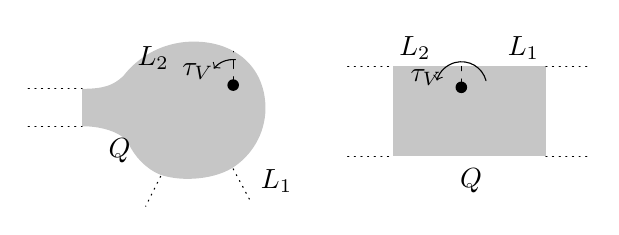
\begin{tikzpicture}[line cap=round,line join=round,scale=0.95]
\begin{scope}
  \path[fill=gray!45] (0,1.45) .. controls (0.3,1.45) and (0.42,1.5) .. (0.55,1.62)
    .. controls (0.75,1.88) and (1.1,2.1) .. (1.55,2.08)
    .. controls (2.05,2.06) and (2.42,1.75) .. (2.45,1.25)
    .. controls (2.47,0.9) and (2.3,0.6) .. (2.05,0.42)
    .. controls (1.8,0.24) and (1.35,0.2) .. (1.05,0.3)
    .. controls (0.85,0.38) and (0.7,0.55) .. (0.62,0.72)
    .. controls (0.55,0.85) and (0.3,0.95) .. (0,0.95)
    -- cycle;
  \draw[dotted] (-0.72,1.45) -- (0,1.45);
  \draw[dotted] (-0.72,0.95) -- (0,0.95);
  \draw[dotted] (2.02,0.38) -- (2.25,-0.05);
  \draw[dotted] (1.05,0.28) -- (0.85,-0.12);
  \fill (2.02,1.5) circle (2.2pt);
  \draw[dashed] (2.02,1.5) -- (2.02,1.95);
  \draw[->] (2.05,1.84) arc[start angle=85,end angle=140,radius=0.34];
  \node at (1.55,1.68) {$\tau_V$};
  \node at (0.95,1.86) {$L_2$};
  \node at (0.5,0.62) {$Q$};
  \node at (2.6,0.22) {$L_1$};
\end{scope}
\begin{scope}[shift={(4.15,0.55)}]
  \path[fill=gray!45] (0,0) -- (2.05,0) -- (2.05,1.2) -- (0,1.2) -- cycle;
  \draw[dotted] (-0.6,1.2) -- (0,1.2);
  \draw[dotted] (2.05,1.2) -- (2.65,1.2);
  \draw[dotted] (-0.6,0) -- (0,0);
  \draw[dotted] (2.05,0) -- (2.65,0);
  \fill (0.92,0.92) circle (2.2pt);
  \draw[dashed] (0.92,0.92) -- (0.92,1.2);
  \draw[->] (1.25,1.01) arc[start angle=15,end angle=165,radius=0.34];
  \node at (0.45,1.05) {$\tau_V$};
  \node at (0.3,1.44) {$L_2$};
  \node at (1.75,1.44) {$L_1$};
  \node at (1.05,-0.33) {$Q$};
\end{scope}
\end{tikzpicture}
\caption{}\label{fig:auxiliary-complex-pictures}
\end{figure}
$l$ 的构造与 $k$ 的构造极为类似。取三\trPointedDisc{}上带\trBoundaryCondition{}$(Q,L_0,L_1)$ 的平凡\trFibration，把它的入向端\trGluing{}到 $E^d\to S^d$ 的出向端上，得到一个\trFibration{}$E^{l,1}\to S^{l,1}$，它自带\trBoundaryCondition{}$F^{l,1}$ 与一个\trRelative\trPerturbationDatum。另一方面，我们也可以再取三\trPointedDisc{}上的一个平凡\trFibration，这次为其配备的\trBoundaryCondition{}在前两条\trBoundaryComponent{}上分别取常值 $Q$ 与常值 $L_0$，而在第三条上实现从 $\tau_V(L_1)$ 到 $L_2$ 的\trIsotopy。在 $L_0$ 那条分支上标记一个边界点，并在点 $\ast$ 处与带有其标准\trBoundaryCondition{}$F$ 的\trFibration{}$E\to S$ 作\trBoundaryConnectedSum。这给出另一个\trFibration{}$E^{l,0}\to S^{l,0}$，\cref{thm:cochain-level-vanishing}如同前面那样适用于它。二者之间有一个显而易见的\trFamily{}$E^{l,r}\to S^{l,r}$ 把它们衔接起来，我们就把 $l$ 取为从相应的\trParametrization{}\trModuliSpace{}得到的\trInvariant（见\cref{fig:l-families}）。
